%%%%%%%%%%%%%%%%%%%%%%%%%%%%%%%%%%%%%%%%%%%%%%%%%%%%%%%%%%%%%%%
%% OXFORD THESIS TEMPLATE

% Use this template to produce a standard thesis that meets the Oxford University requirements for DPhil submission
%
% Originally by Keith A. Gillow (gillow@maths.ox.ac.uk), 1997
% Modified by Sam Evans (sam@samuelevansresearch.org), 2007
% Modified by John McManigle (john@oxfordechoes.com), 2015
% Modified by Ulrik Lyngs (ulrik.lyngs@cs.ox.ac.uk), 2018-, for use with R Markdown
%
% Ulrik Lyngs, 25 Nov 2018: Following John McManigle, broad permissions are granted to use, modify, and distribute this software
% as specified in the MIT License included in this distribution's LICENSE file.
%
% John commented this file extensively, so read through to see how to use the various options.  Remember that in LaTeX,
% any line starting with a % is NOT executed.

%%%%% PAGE LAYOUT
% The most common choices should be below.  You can also do other things, like replace "a4paper" with "letterpaper", etc.

% 'twoside' formats for two-sided binding (ie left and right pages have mirror margins; blank pages inserted where needed):
%\documentclass[a4paper,twoside]{templates/ociamthesis}
% Specifying nothing formats for one-sided binding (ie left margin > right margin; no extra blank pages):
%\documentclass[a4paper]{ociamthesis}
% 'nobind' formats for PDF output (ie equal margins, no extra blank pages):
%\documentclass[a4paper,nobind]{templates/ociamthesis}

% As you can see from the line below, oxforddown uses the a4paper size, 
% and passes in the binding option from the YAML header in index.Rmd:
\documentclass[a4paper, nobind]{templates/ociamthesis}


%%%%% ADDING LATEX PACKAGES
% add hyperref package with options from YAML %
\usepackage[pdfpagelabels]{hyperref}
% handle long urls
\usepackage{xurl}
% change the default coloring of links to something sensible
\usepackage{xcolor}

\definecolor{mylinkcolor}{RGB}{0,0,139}
\definecolor{myurlcolor}{RGB}{0,0,139}
\definecolor{mycitecolor}{RGB}{0,33,71}

\hypersetup{
  hidelinks,
  colorlinks,
  linktocpage=true,
  linkcolor=mylinkcolor,
  urlcolor=myurlcolor,
  citecolor=mycitecolor
}


% add float package to allow manual control of figure positioning %
\usepackage{float}

% enable strikethrough
\usepackage[normalem]{ulem}

% use soul package for correction highlighting
\usepackage{color, soulutf8}
\definecolor{correctioncolor}{HTML}{CCCCFF}
\sethlcolor{correctioncolor}
\newcommand{\ctext}[3][RGB]{%
  \begingroup
  \definecolor{hlcolor}{#1}{#2}\sethlcolor{hlcolor}%
  \hl{#3}%
  \endgroup
}
% stop soul from freaking out when it sees citation commands
\soulregister\ref7
\soulregister\cite7
\soulregister\citet7
\soulregister\autocite7
\soulregister\textcite7
\soulregister\pageref7

%%%%% FIXING / ADDING THINGS THAT'S SPECIAL TO R MARKDOWN'S USE OF LATEX TEMPLATES
% pandoc puts lists in 'tightlist' command when no space between bullet points in Rmd file,
% so we add this command to the template
\providecommand{\tightlist}{%
  \setlength{\itemsep}{0pt}\setlength{\parskip}{0pt}}
 
% allow us to include code blocks in shaded environments

% User-included things with header_includes or in_header will appear here
% kableExtra packages will appear here if you use library(kableExtra)
\usepackage{booktabs}
\usepackage{longtable}
\usepackage{array}
\usepackage{multirow}
\usepackage{wrapfig}
\usepackage{float}
\usepackage{colortbl}
\usepackage{pdflscape}
\usepackage{tabu}
\usepackage{threeparttable}
\usepackage{threeparttablex}
\usepackage[normalem]{ulem}
\usepackage{makecell}
\usepackage{xcolor}


%UL set section header spacing
\usepackage{titlesec}
% 
\titlespacing\subsubsection{0pt}{24pt plus 4pt minus 2pt}{0pt plus 2pt minus 2pt}


%UL set whitespace around verbatim environments
\usepackage{etoolbox}
\makeatletter
\preto{\@verbatim}{\topsep=0pt \partopsep=0pt }
\makeatother


%%%%%%% PAGE HEADERS AND FOOTERS %%%%%%%%%
\usepackage{fancyhdr}
\setlength{\headheight}{15pt}
\fancyhf{} % clear the header and footers
\pagestyle{fancy}
\renewcommand{\chaptermark}[1]{\markboth{\thechapter. #1}{\thechapter. #1}}
\renewcommand{\sectionmark}[1]{\markright{\thesection. #1}} 
\renewcommand{\headrulewidth}{0pt}





% UL page number position 
\fancyfoot[C]{\emph{\thepage}} %regular pages
\fancypagestyle{plain}{\fancyhf{}\fancyfoot[C]{\emph{\thepage}}} %chapter pages




%%%%% SELECT YOUR DRAFT OPTIONS
% This adds a "DRAFT" footer to every normal page.  (The first page of each chapter is not a "normal" page.)

% IP feb 2021: option to include line numbers in PDF

% for line wrapping in code blocks
\usepackage{fancyvrb}
\usepackage{fvextra}
\DefineVerbatimEnvironment{Highlighting}{Verbatim}{breaklines=true, breakanywhere=true, commandchars=\\\{\}}

% This highlights (in blue) corrections marked with (for words) \mccorrect{blah} or (for whole
% paragraphs) \begin{mccorrection} . . . \end{mccorrection}.  This can be useful for sending a PDF of
% your corrected thesis to your examiners for review.  Turn it off, and the blue disappears.


%%%%% BIBLIOGRAPHY SETUP
% Note that your bibliography will require some tweaking depending on your department, preferred format, etc.
% If you've not used LaTeX before, I recommend just using pandoc for citations -- this is what's used unless you specific e.g. "citation_package: natbib" in index.Rmd
% If you're already a LaTeX pro and are used to natbib or something, modify as necessary.

% this allows the latex template to handle pandoc citations




% Uncomment this if you want equation numbers per section (2.3.12), instead of per chapter (2.18):
%\numberwithin{equation}{subsection}


%%%%% THESIS / TITLE PAGE INFORMATION
% Everybody needs to complete the following:




% Master's candidates who require the alternate title page (with candidate number and word count)
% must also un-comment and complete the following three lines:

% Uncomment the following line if your degree also includes exams (eg most masters):
%\renewcommand{\submittedtext}{Submitted in partial completion of the}
% Your full degree name.  (But remember that DPhils aren't "in" anything.  They're just DPhils.)


% Term and year of submission, or date if your board requires (eg most masters)



%%%%% YOUR OWN PERSONAL MACROS
% This is a good place to dump your own LaTeX macros as they come up.

% To make text superscripts shortcuts
\renewcommand{\th}{\textsuperscript{th}} % ex: I won 4\th place
\newcommand{\nd}{\textsuperscript{nd}}
\renewcommand{\st}{\textsuperscript{st}}
\newcommand{\rd}{\textsuperscript{rd}}

%%%%% THE ACTUAL DOCUMENT STARTS HERE
\begin{document}

%%%%% CHOOSE YOUR LINE SPACING HERE
% This is the official option.  Use it for your submission copy and library copy:
\setlength{\textbaselineskip}{22pt plus2pt}
% This is closer spacing (about 1.5-spaced) that you might prefer for your personal copies:
%\setlength{\textbaselineskip}{18pt plus2pt minus1pt}

% You can set the spacing here for the roman-numbered pages (acknowledgements, table of contents, etc.)
\setlength{\frontmatterbaselineskip}{17pt plus1pt minus1pt}

% UL: You can set the line and paragraph spacing here for the separate abstract page to be handed in to Examination schools
\setlength{\abstractseparatelineskip}{13pt plus1pt minus1pt}
\setlength{\abstractseparateparskip}{0pt plus 1pt}

% UL: You can set the general paragraph spacing here - I've set it to 2pt (was 0) so
% it's less claustrophobic
\setlength{\parskip}{2pt plus 1pt}

%
% Customise title page
%
\def\crest{}
\renewcommand{\university}{}
\renewcommand{\submittedtext}{}
\renewcommand{\thesistitlesize}{\fontsize{22pt}{28pt}\selectfont}
\renewcommand{\gapbeforecrest}{25mm}
\renewcommand{\gapaftercrest}{25mm
}


% Leave this line alone; it gets things started for the real document.
\setlength{\baselineskip}{\textbaselineskip}


%%%%% CHOOSE YOUR SECTION NUMBERING DEPTH HERE
% You have two choices.  First, how far down are sections numbered?  (Below that, they're named but
% don't get numbers.)  Second, what level of section appears in the table of contents?  These don't have
% to match: you can have numbered sections that don't show up in the ToC, or unnumbered sections that
% do.  Throughout, 0 = chapter; 1 = section; 2 = subsection; 3 = subsubsection, 4 = paragraph...

% The level that gets a number:
\setcounter{secnumdepth}{2}
% The level that shows up in the ToC:
\setcounter{tocdepth}{1}


%%%%% ABSTRACT SEPARATE
% This is used to create the separate, one-page abstract that you are required to hand into the Exam
% Schools.  You can comment it out to generate a PDF for printing or whatnot.

% JEM: Pages are roman numbered from here, though page numbers are invisible until ToC.  This is in
% keeping with most typesetting conventions.
\begin{romanpages}

% Title page is created here

%%%%% DEDICATION

%%%%% ACKNOWLEDGEMENTS


%%%%% ABSTRACT


%%%%% MINI TABLES
% This lays the groundwork for per-chapter, mini tables of contents.  Comment the following line
% (and remove \minitoc from the chapter files) if you don't want this.  Un-comment either of the
% next two lines if you want a per-chapter list of figures or tables.
\dominitoc % include a mini table of contents

% This aligns the bottom of the text of each page.  It generally makes things look better.
\flushbottom

% This is where the whole-document ToC appears:


% Uncomment to generate a list of tables:
%%%%% LIST OF ABBREVIATIONS
% This example includes a list of abbreviations.  Look at text/abbreviations.tex to see how that file is
% formatted.  The template can handle any kind of list though, so this might be a good place for a
% glossary, etc.

% The Roman pages, like the Roman Empire, must come to its inevitable close.
\end{romanpages}

%%%%% CHAPTERS
% Add or remove any chapters you'd like here, by file name (excluding '.tex'):
\flushbottom

% all your chapters and appendices will appear here
\hypertarget{rmd-basics}{%
\chapter{Results}\label{rmd-basics}}

\minitoc 

\noindent

\hypertarget{participants-characteristics}{%
\section{Participants' Characteristics}\label{participants-characteristics}}

When participants were asked the amount of time they have used a chatbot
in any form or subject, 23 stated they had never used a chatbot.
Further, 19/42 stated having used a chatbot at least once for between
0-4 hours of use in total. These are likely commercial/website- based
assistant chatbots however there are some medical/healthcare resources
known to be used in anatomy and/or patient interactions. One individual
had spent much longer time with usage- this was the mature student.

\begin{longtable}[]{@{}lr@{}}
\caption{Previous Chatbot Usage of Participants\\
}\tabularnewline
\toprule()
Previous\_Chatbot\_Usage & n \\
\midrule()
\endfirsthead
\toprule()
Previous\_Chatbot\_Usage & n \\
\midrule()
\endhead
1-4 hours & 16 \\
10-19 hours & 1 \\
5-9 hours & 2 \\
Never & 23 \\
\bottomrule()
\end{longtable}

In short, approximately 50\% had never used a chatbot, and 45\% had used a
chatbot, at some period over the years, for a short period of time.

Most learners use books or online books as resources. They may use multiple sources however they were asked to note the primary source. Only 6 stated their primary sources were \emph{Online videos/interactive materials} which includes such tools as chatbots.

\begin{figure}
\centering
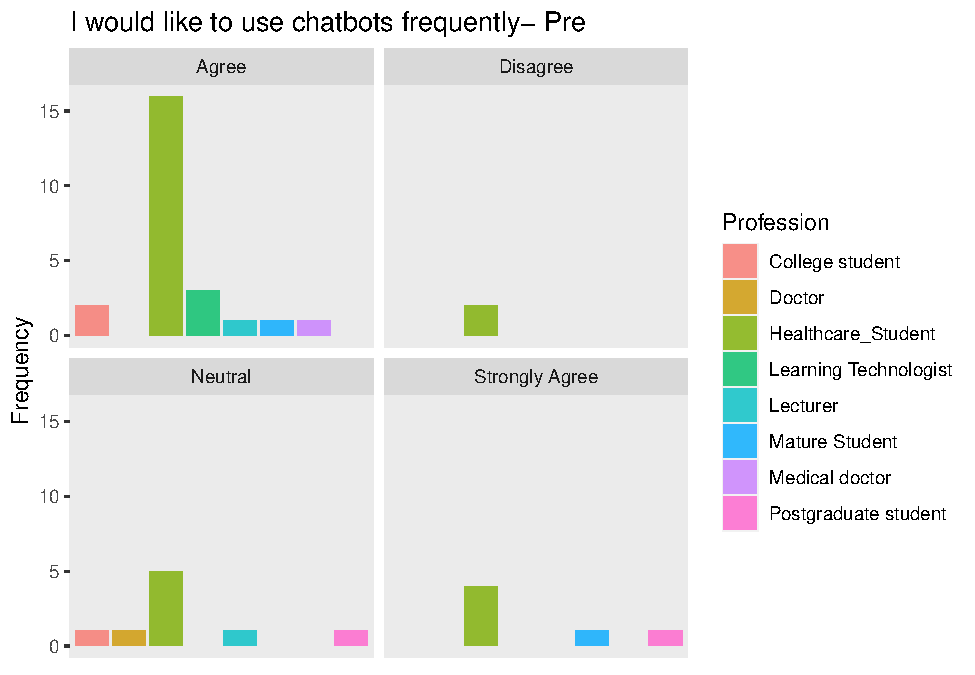
\includegraphics{02-Results_files/figure-latex/Boxplotsplits2-1.pdf}
\caption{\label{fig:Boxplotsplits2}Chatbot Usage History- Pre}
\end{figure}

The first boxplot (\ref{fig:Boxplotsplits2}) shows learners perceptions of easy of use of mobile app and other educational mobile resources

\begin{figure}
\centering
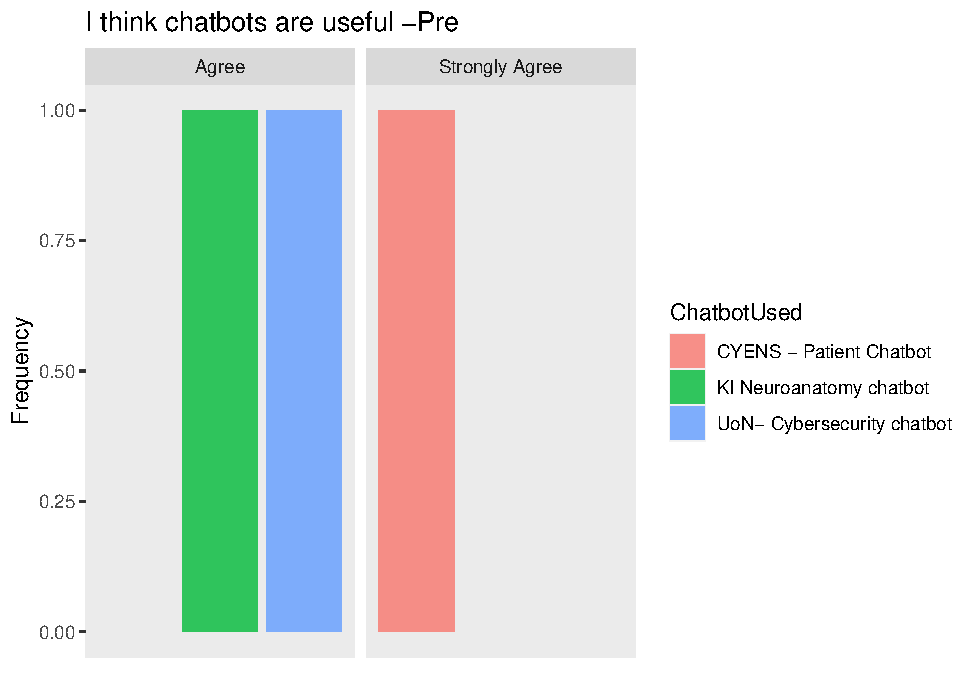
\includegraphics{02-Results_files/figure-latex/BoxplotUsefulPre-1.pdf}
\caption{\label{fig:BoxplotUsefulPre}Chatbots are Useful Opinion- Pre}
\end{figure}

(\ref{fig:BoxplotUsefulPre}) shows the opinions of all participants on the usefulness of chatbots. Many had not had experience with them yet had positive rating.

This positive opinions of chatbots may be from colleagues, friends, media, tutors, or other social information of the benefits in healthcare education. Around 25\% were neutral or disagreed that healthcare chatbots were useful.

\textbf{\emph{The participants then used the 4 chatbots, and completed the
post-usage survey after each chatbot. Results after use are as
followed:}}

\strut \\

\hypertarget{chatbot-usability-questionnaire-cuq}{%
\section{Chatbot Usability Questionnaire (CUQ)}\label{chatbot-usability-questionnaire-cuq}}

\hypertarget{cuq-calculation-tool}{%
\subsection{CUQ Calculation tool}\label{cuq-calculation-tool}}

The CUQ was developed by researchers at Ulster University,
\href{https://www.ulster.ac.uk/research/topic/computer-science/artificial-intelligence/projects/cuq}{Link}
and as the calculation can be complex, a dedicated calculation tool has been created.

Please download the CEPEH CUQ calculation tool which has all of the data entered, so you can see the CEPEH CUQ scoring

\href{CUQ-Calculation-Tool.xlsx}{Click here to download CUQ calc tool}

\href{cuq.png}{Click here to download CEPEH CUQ score result}

\begin{figure}

{\centering 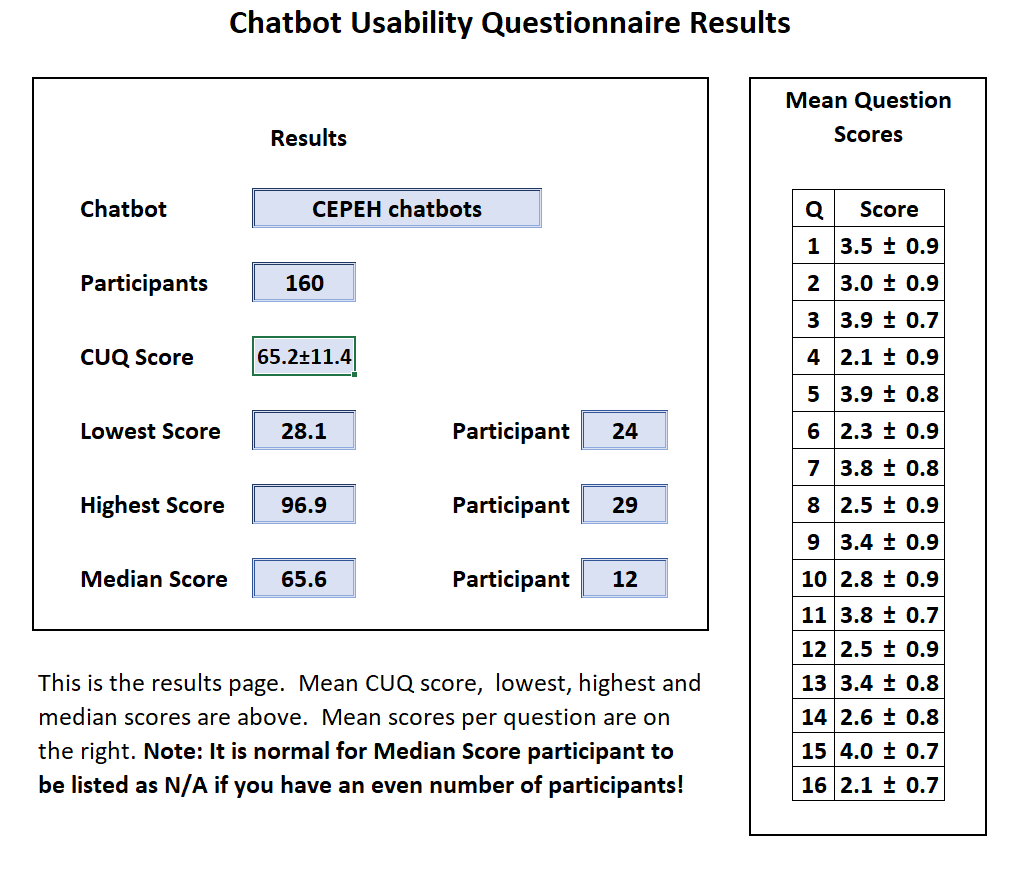
\includegraphics[width=0.75\linewidth]{cuq} 

}

\caption{CUQ CEPEH Score}\label{fig:cuqimage}
\end{figure}

Although the design and development was similar, each chatbot CUQ score was calculated to understand how the topic content may affect usability:

The breakdown of the chatbots was:

\begin{itemize}
\tightlist
\item
  Aristotle University of Thessaloniki CUQ score = 63/100
\item
  CYENS Centre of Excellence CUQ score = 67/100
\item
  Karolinska Institute CUQ score = 63/100
\item
  University of Nottingham CUQ score = 68/100
\end{itemize}

The score for all 3 chatbots grouped was 65/100. See Discussion CUQ
section for interpretation

\begin{figure}

{\centering 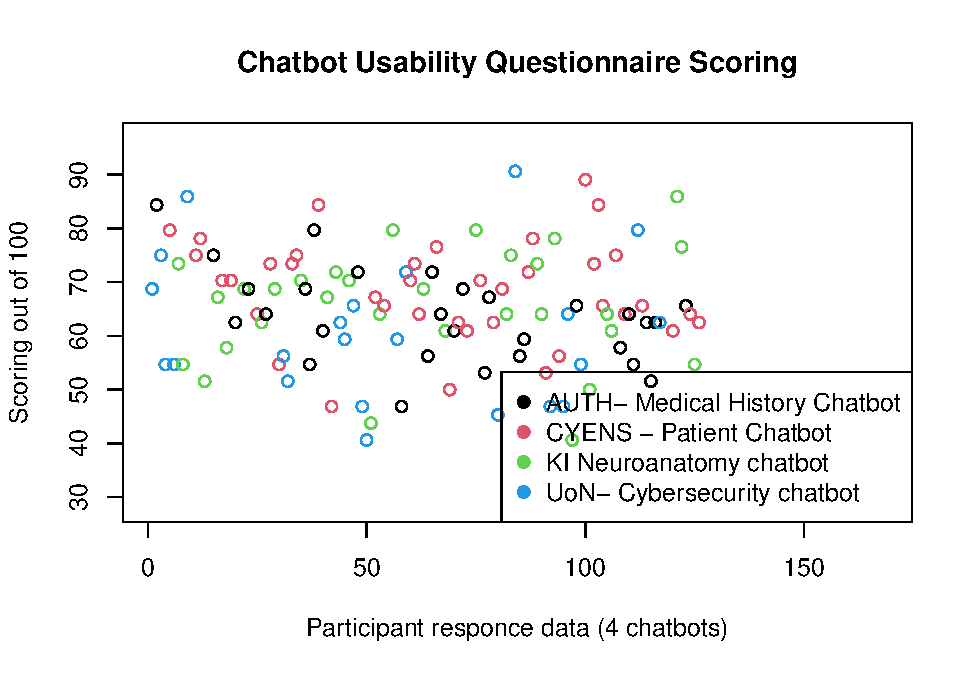
\includegraphics{02-Results_files/figure-latex/CUQscatterplot-1} 

}

\caption{CUQ Scatter Plot}\label{fig:CUQscatterplot}
\end{figure}

Figure (\ref{fig:CUQscatterplot}) shows the CUQ scores as a scatter plot to highlight how there was a moderate distribution of results.
Further exploration is required to understand which elements are causing this spread, and if it was due to problems within a small group of learners.

\hypertarget{system-usability-scale-sus-scores}{%
\section{System Usability Scale (SUS) Scores}\label{system-usability-scale-sus-scores}}

\emph{Note= The amount of `agreement' is defined as the addition of `Agree'
and `Strongly agree' responses.}

The SUS score should consist of 10 items. However, some SUS questions were improved upon by 1 or more CUQ questions, specifically to this Chatbot study. The SUS results would be obscured by the CUQ scores, expect 2 that did not have cross-over. The two questions were:

\begin{itemize}
\tightlist
\item
  I would like to use the CEPEH chatbot I tested, more frequently
  (SUS1)(post)
\item
  I felt confident using the CEPEH chatbot (SUS2)(post)
\end{itemize}

This meant the score of the SUS was not created, however the CUQ score better represented the Learners' perceptions of the CEPEH chatbot in terms of feasibility of use and acceptability in healthcare curricula.

\begin{longtable}[]{@{}lr@{}}
\toprule()
Keep Using CEPEH Chatbot & Responces \\
\midrule()
\endhead
Agree & 66 \\
Disagree & 15 \\
Neutral & 17 \\
Not Applicable & 3 \\
Strongly Agree & 23 \\
Strongly Disagree & 2 \\
\bottomrule()
\end{longtable}

The table @ref(tab:SUS keepusing) above shows the results for agreement participants may
continue to use the CEPEH chatbots: 89/126 (70\%) agreed or strongly
agreed. However, there were 23 records that learners were neutral or
disagree they would continue use.

\begin{longtable}[]{@{}lr@{}}
\toprule()
Confidence using CEPEH Chatbot(s) & Responces \\
\midrule()
\endhead
Agree & 71 \\
Disagree & 11 \\
Neutral & 21 \\
Not Applicable & 4 \\
Strongly Agree & 19 \\
\bottomrule()
\end{longtable}

Confidence when using the chatbots is in table \ref{tab:confidence}- it shows the distribution of agreement for participants for all
4 chatbots. The table shows 90/126 records that participants feel they
are confident in using the chatbots. However, 21/126 (16\%) were neutral
and 11/126 (8.5\%) disagreed and this was explored in the qualitative
analysis section.

\hypertarget{technology-acceptance-model}{%
\section{Technology Acceptance Model}\label{technology-acceptance-model}}

The TAM questions were analysed according to their subsets. The subsets
were Perceived Usefulness (PU) and Perceived Easy of Use (PEU)

The questions were: Perceived Usefulness (PU)

\begin{enumerate}
\def\labelenumi{\arabic{enumi}.}
\tightlist
\item
  Using CEPEH chatbots would enable me to accomplish tasks more
  quickly
\item
  Using CEPEH chatbots would increase performance
\item
  Using CEPEH chatbots would increase my productivity
\item
  I would find CEPEH chatbots useful on my course
\end{enumerate}

Perceived Easy of Use (PEU)

\begin{enumerate}
\def\labelenumi{\arabic{enumi}.}
\setcounter{enumi}{4}
\tightlist
\item
  Learning to use CEPEH chatbots would be easy to me
\item
  It would be easy for me to be skilful at using CEPEH chatbots
\item
  My interactions with CEPEH chatbots would be clear and
  understandable
\item
  I would find CEPEH chatbots easy to use
\end{enumerate}

\emph{Results}

The scores as a percentage of agreement, were calculated by averaging
the subsets and interpreted as:

\begin{itemize}
\item
  Before using the CEPEH chatbots, there was 66\% (2.2/5) agreement for
  the Perceived Usefulness of chatbots in healthcare education, and
  after 48\% (2.6/5) agreed.
\item
  Before using the CEPEH chatbots, there was 64\% (2.3) agreement for
  Perceived Ease of Use of chatbots in healthcare education, and after
  51\% (2.56) agreed.
\end{itemize}

The justification for this may be due to being early versions of
applications with limited functionality and functions which can be
difficult for user to experience the intended further range of features
and learning exercises.

\begin{figure}

{\centering 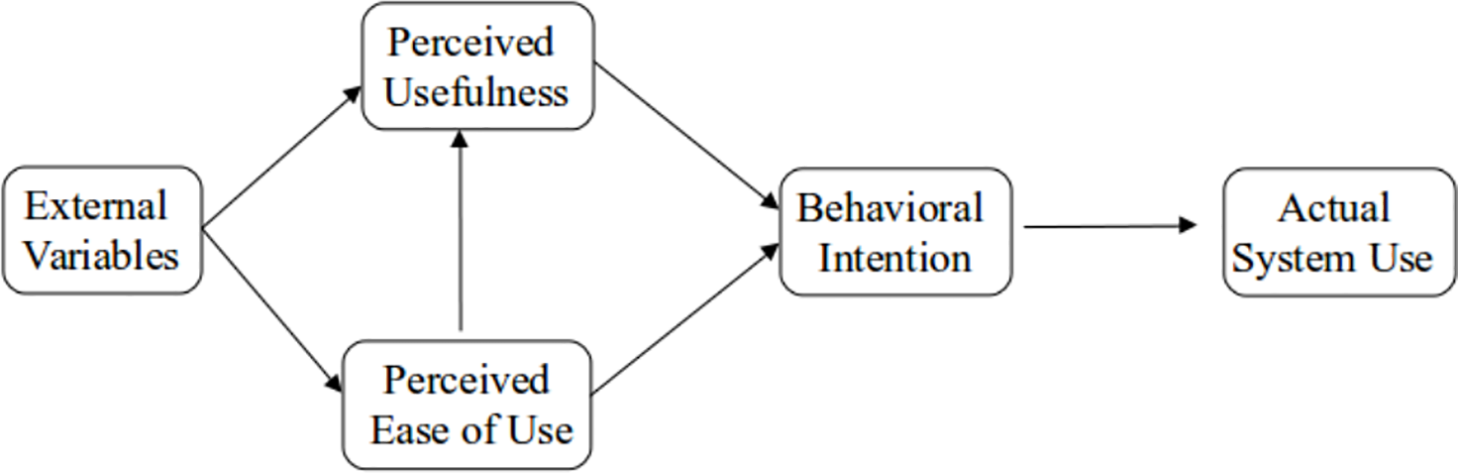
\includegraphics[width=0.75\linewidth]{tam1} 

}

\caption{TAM Model processes}\label{fig:tam}
\end{figure}

\hypertarget{other-measures}{%
\section{Other Measures}\label{other-measures}}

\hypertarget{knowledge-of-topics-after-use}{%
\subsection{Knowledge of Topics after Use}\label{knowledge-of-topics-after-use}}

\begin{figure}
\centering
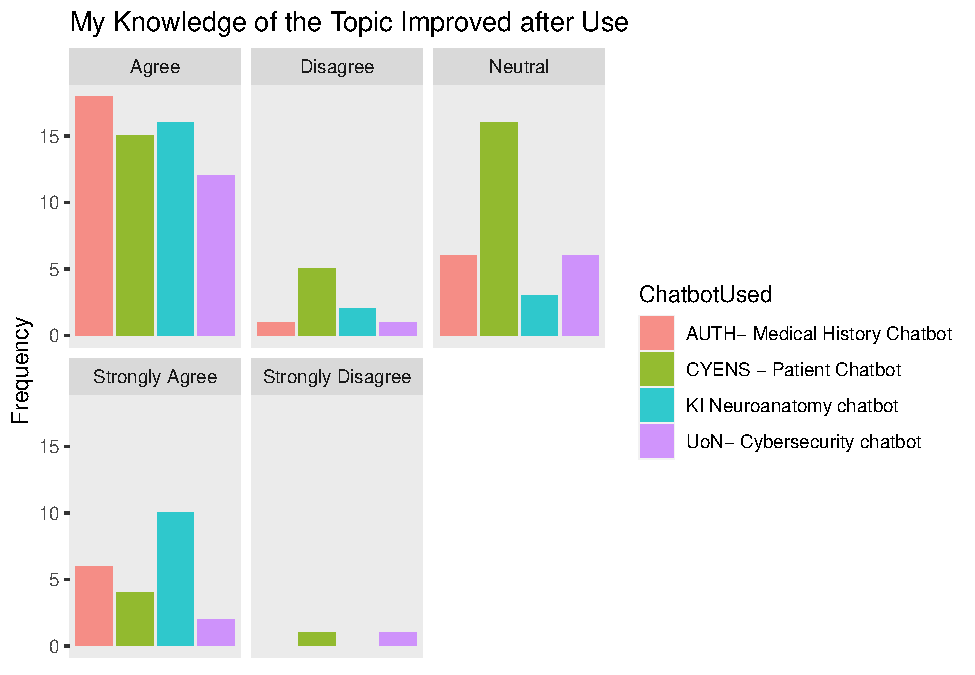
\includegraphics{02-Results_files/figure-latex/Boxplotsplits5-1.pdf}
\caption{\label{fig:Boxplotsplits5}Improvements in Knowledge}
\end{figure}

CYENS chatbot had around 10 more participants stating that they were
neutral on gaining knowledge of the topic

\hypertarget{trust-in-cepeh-chatbots-after-use}{%
\subsection{Trust in CEPEH chatbots after Use}\label{trust-in-cepeh-chatbots-after-use}}

\begin{figure}
\centering
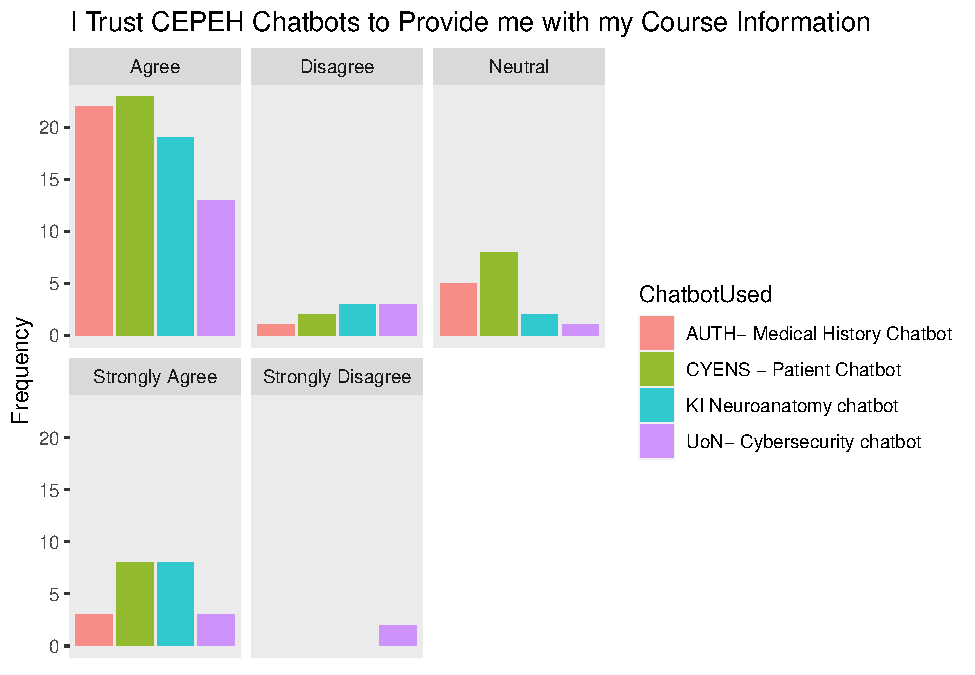
\includegraphics{02-Results_files/figure-latex/Boxplotsplits6-1.pdf}
\caption{\label{fig:Boxplotsplits6}Trust Chatbots POST use}
\end{figure}

The figure above, (\ref{fig:Boxplotsplits6}) shows the ratings by
participants of the CEPEH Chatbots to provide them with the necessary
course information. This is a integral element in learners' motivational
and educational choices to reuse the learning resources. As previously
described, the trust of the information is also a factor in these
responses.

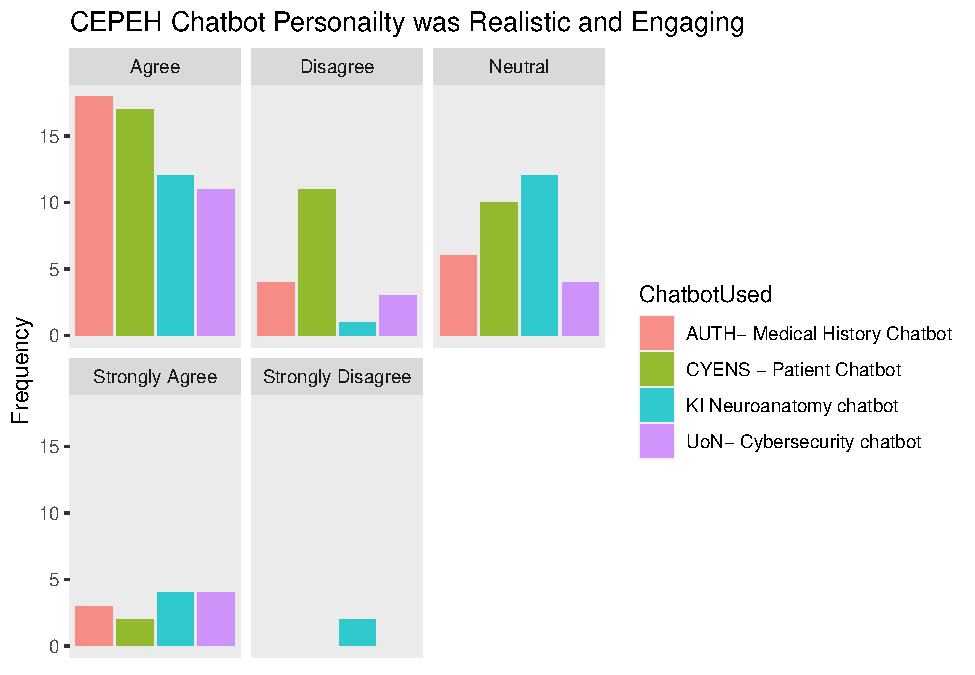
\includegraphics{02-Results_files/figure-latex/Boxplotsplits7-1.pdf}

There was mixed results for the chatbot used being realistic and
engaging. This question has two descriptive terms however based on the
other results we understand that the chatbots' NLP logic, or ability to
respond required improvement to be more `smooth' in replying. The
primary limitation was found in the `robotic' interactions(See Figure
10). This was investigated further in the `Text Mining' and `Sentiment
Analysis' sections.

\hypertarget{personality-and-interactions}{%
\subsection{Personality and Interactions}\label{personality-and-interactions}}

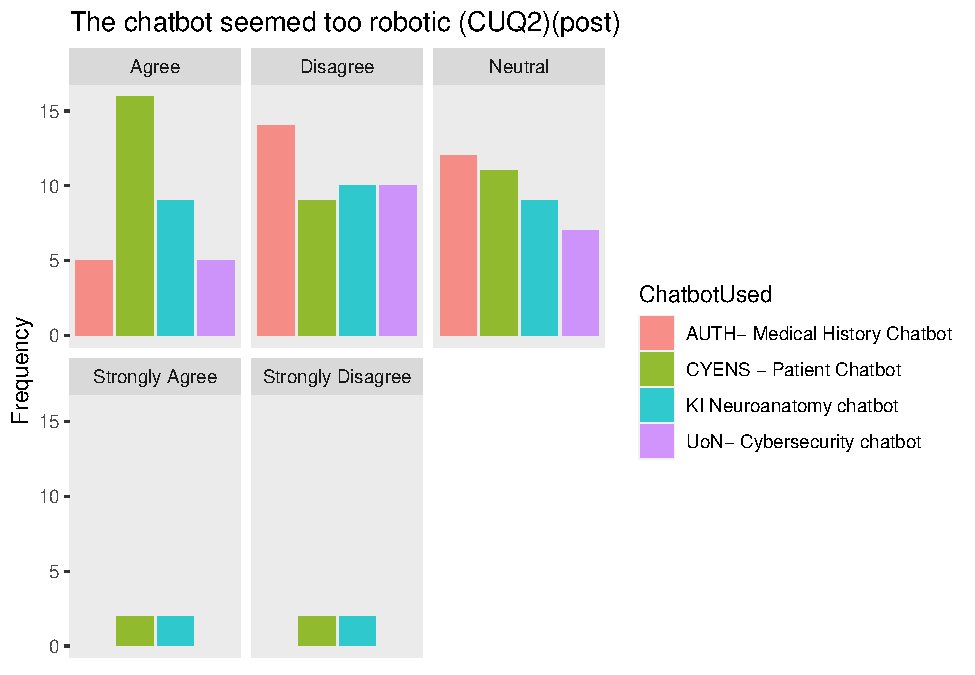
\includegraphics{02-Results_files/figure-latex/Boxplotsplits8-1.pdf}

\emph{The chatbot seemed too robotic} results had the largest mix of
responses, and for all 4 chatbots evaluated. The University of
Nottingham Cybersecurity chatbot had more deterministic pathways with
exploitation of the NLP modelling to provide illusion of realism. This
may explain why there was less agreement. However, Neutrality and/or
agreement was not desired.

\hypertarget{ease-of-use-and-seeking-support}{%
\subsection{Ease of Use and Seeking Support}\label{ease-of-use-and-seeking-support}}

\begin{figure}
\centering
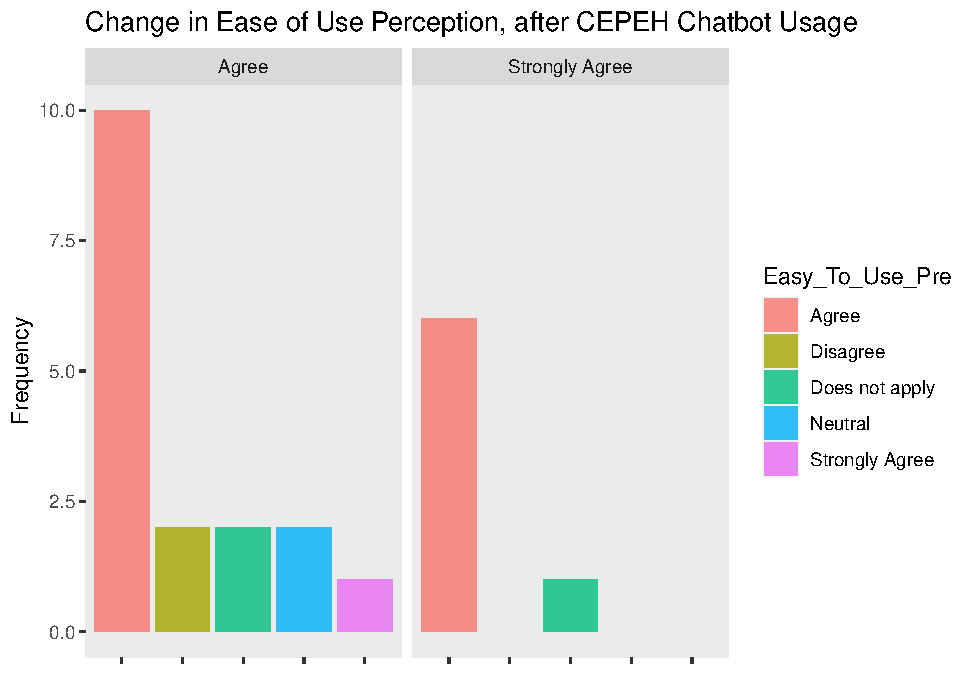
\includegraphics{02-Results_files/figure-latex/Boxplotsplits9-1.pdf}
\caption{\label{fig:Boxplotsplits9}Ease of Use Comparison}
\end{figure}

After usage, there was only agreement in Ease of Use- as shown in
(\ref{fig:Boxplotsplits9} as there are no `Neutral' or disagree
columns. Any learners with disagreement before using the CEPEH chatbots,
after believed they were easy to use.

\begin{figure}
\centering
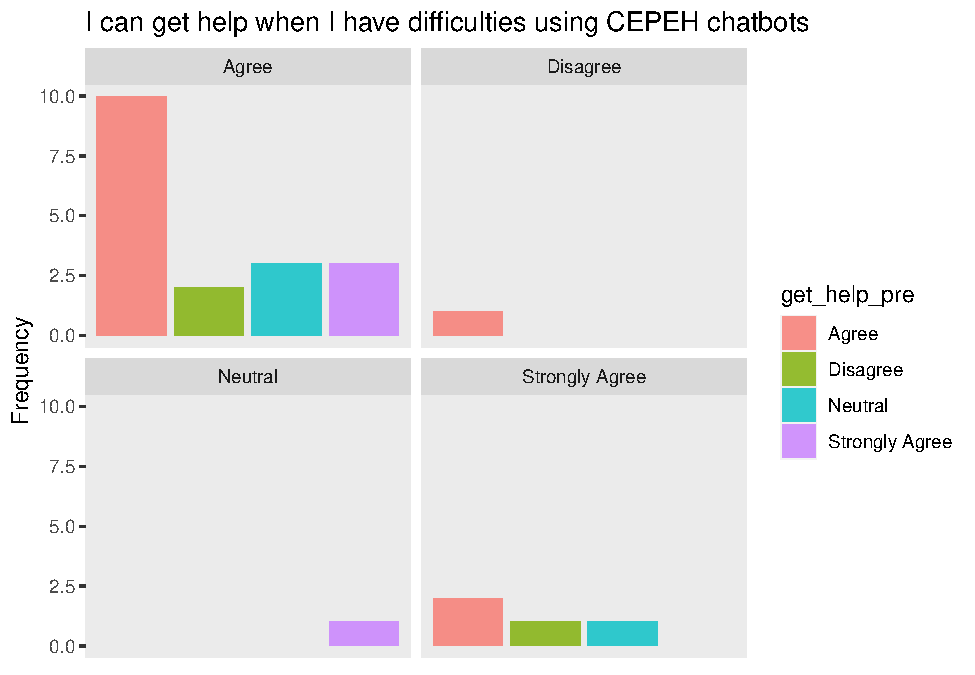
\includegraphics{02-Results_files/figure-latex/Boxplotsplits10-1.pdf}
\caption{\label{fig:Boxplotsplits10}Ease of Use Comparison}
\end{figure}

Those who disagreed or were neutral in the pre usage measure, improved
their understanding that help was available with the CEPEH chatbots.
After usage, 40 participants agreed they could get help if they had
difficulty using the resources.

\hypertarget{inferential-statistics}{%
\section{Inferential Statistics}\label{inferential-statistics}}

\hypertarget{repeated-measures-t-test-results}{%
\subsection{Repeated Measures T-test results}\label{repeated-measures-t-test-results}}

After using the CEPEH chatbots, majority of participants stated they
would reuse the chatbots. However, there was 6 counts of \emph{disagree} or
\emph{strongly disagree} for all 4 chatbots. Further, there were 17 counts of
neutral in reuse, which was approximately 4 participants per chatbot
(see (\ref{fig:Boxplotsplits4}).

\begin{figure}
\centering
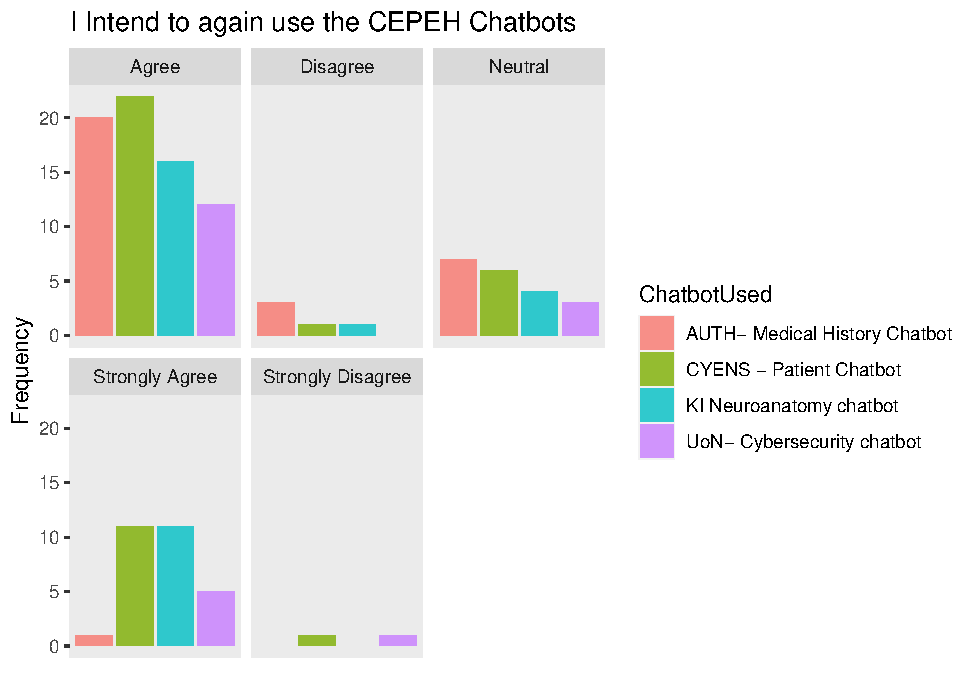
\includegraphics{02-Results_files/figure-latex/Boxplotsplits4-1.pdf}
\caption{\label{fig:Boxplotsplits4}Intend to Reuse-Post}
\end{figure}

For CYENS, even though the knowledge of the topic was not perceived to
improve by some participants, this box plot shows how 34/42 stated they
would reuse the chatbot developed by CYENS.

\begin{figure}
\centering
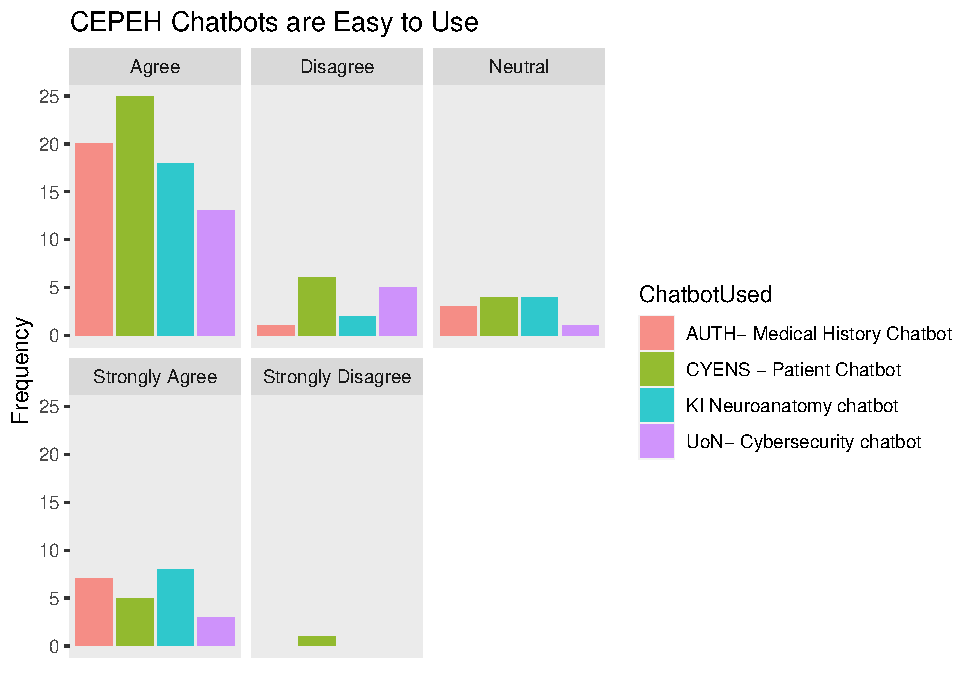
\includegraphics{02-Results_files/figure-latex/Boxplotsplits3-1.pdf}
\caption{\label{fig:Boxplotsplits3}Easy to Use- Post}
\end{figure}

There was only 1 `Strongly Disagree' response. The agreement options
counted for the majority of the data.

\hypertarget{other-findings}{%
\section{Other Findings}\label{other-findings}}

Other questions

I intend to continue using chatbots in the future (BI1)

The chatbot provided the information I needed with minimal commands

My knowledge of the topic improved after i had used the Chatbot

My confidence in understanding the topic improved after I had used the
Chatbot

The chatbot provided me with the type of response i expected from asking
a tutor/lecturer

The information provided was reliable

The chatbot has a high level of trustworthiness

The duration of conversations to find my answer was too long

The videos/images provided were useful to my questions

The chatbot exceeded my expectation of how it could help me

The chatbot exceeded my expectation of how it could engage with me

I think this learning method could help me to acquire knowledge

I would use this tool again as it has some value to me

I think I will actively use this learning method

I believe I had some choice about learning during chatbot use

I would trust the chatbot to provide me with information for my course

One piece of knowledge I learned from the chatbot was..

Repeated Measures t-test, aka paired t-test (before and after
measurements)

This t-test compares confident using mobile chatbots before and after
CEPEH chatbot usage.

%%%%% REFERENCES


\end{document}
